%&pdflatex
\documentclass[11pt]{article}
\usepackage{url,enumerate, amssymb, amsfonts}
\usepackage[colorlinks = true,
linkcolor = blue,
urlcolor  = blue,
citecolor = green,
anchorcolor = blue]{hyperref}
%\usepackage{setspace,listings}
\usepackage{graphicx}
\usepackage{amsmath}
\usepackage{psfrag}
\usepackage[font=small,labelfont=bf]{caption}
\usepackage{enumerate}
\usepackage{authblk}
\usepackage[sort&compress,comma,square,numbers]{natbib}
\usepackage{url} % not cruci
%\pdfminorversion=4
\usepackage{setspace}
\usepackage{lscape}
\usepackage{color,amssymb}
\usepackage{mathtools}
\usepackage{dcolumn}
\usepackage{indentfirst, verbatim, float}
\usepackage[margin=1.2in]{geometry}
%\newcounter{equationset, sectsty, breqn}
%\usepackage{setspace, amsmath,color}
%\usepackage{color,amssymb}
\usepackage{mathtools, amsthm, subcaption}
\theoremstyle{definition}
\newtheorem{definition}{Definition}[section]
\newtheorem{theorem}{Theorem}[section]
\newtheorem{corollary}{Corollary}[theorem]
\newtheorem{lemma}[theorem]{Lemma}
\newtheorem{remark}{Remark}
\bibliographystyle{plainnat}
\usepackage{sidecap}
\usepackage{titlesec}
\sidecaptionvpos{figure}{c}

% NOTE: To produce unblinded version, replace "0" with "1" below.
\newcommand{\blind}{1}
% DON'T change margins - should be 1 inch all around.
\newcommand{\cs}[1]{\textcolor{blue}{cs: #1}}

\begin{document}

\def\spacingset#1{\renewcommand{\baselinestretch}%
{#1}\small\normalsize} \spacingset{1}

%%%%%%%%%%%%%%%%%%%%%%%%%%%%%%%%%%%%%%%%%%%%%%%%%%%%%%%%%%%%%%%%%%%%%%%%%%%%%%
\title{\bf Nonparametric Network Dependence Testing by Diffusion Distance}
\if1\blind
{\author[1]{Youjin Lee (ylee160@jhu.edu)} %\thanks{cshen6@jhu.edu}}
	\author[2]{Cencheng Shen} %\thanks{cshen6@jhu.edu}}
	\author[2,3,4]{Joshua T. Vogelstein}
	\affil[1]{Department of Biostatistics, Johns Hopkins University}
  \affil[2]{Center for Imaging Science, Johns Hopkins University}
  \affil[3]{Department of Biomedical Engineering and Institute for Computational Medicine, Johns Hopkins University}
  \affil[4]{Institute for Data-Intensive Engineering \& Science, Johns Hopkins University}
	\maketitle
} \fi

	\if0\blind
	{
		\bigskip
		\bigskip
		\bigskip
		\begin{center}
			{\LARGE\bf Nonparametric Network Dependence Testing By Diffusion Maps}
		\end{center}
		\medskip
	} \fi

\begin{abstract}
%The text of your abstract. 200 or fewer words.
Investigating how network structures are associated with nodal attributes of interest is a core problem in network science. As the network topology is a structured and often high-dimensional object, many traditional nonparametric tests are no longer applicable and parametric approaches are dominant in graph inferences. Here we propose a new procedure to testing dependence between graphs and attributes, via diffusion distances and distance-based correlation testing. We demonstrate that our nonparametric method not only yields a consistent test statistic under common network models, but also significantly surpasses the testing power of existing benchmarks under various circumstances. 
\end{abstract}

\noindent%
{\it Keywords:} testing independence, exchangeable graph, diffusion distance, distance correlation, multiscale generalized correlation

\sloppy
\doublespacing

\section{Introduction}
\label{sec:intro}
	\vspace*{-0.2cm}
	% General Backgrounds
Propelled by increasing demand and supply of graph data from various disciplines, the ubiquitous influence of network inferences has motivated numerous recent advances and applications in statistics, physics, computer science, biology, social science, etc., which further poses many new challenges to data scientists. One of the most fundamental statistical questions is to determine and characterize the relationship among multiple modalities of a given data set, for which the first step is to test the existence of any dependency. However, the lack of a principal notion of correlation in the graph domain has not only hindered the progress of nonparametric dependency testing methods, but also deterred a rich literature of statistical techniques in other inferences (e.g., regression, feature screening, two-sample test) from being directly applied to graphs.
 
% Graph data general
Mathematically, a graph (or equivalently a network) $\mathbf{G}=(V,E)$ consists of a set $V$ of nodes (or vertices) together with a set $E$ of edges, which is often represented via an adjacency matrix $\mathbf{A} = \{A_{ij} : i,j= 1,..,n \}$, e.g. for an unweighted and undirected network, $A_{ij} = 1$ if node $i$ and node $j$ are connected by an edge, and zero otherwise. Therefore, $\mathbf{A}$ is a symmetric square matrix that does not satisfy traditional data assumptions, e.g., each observation can be assumed independently and identically distributed, the sample size increases faster than the feature dimension, etc., which is a notable obstacle for directly applying conventional statistical methods. Therefore, graph inferences have long relied on specifying a particular statistical model, such as the Erdos-Renyi model \cite{erdosrenyi1959,Gilbert1959}, stochastic block model~\cite{HollandEtAl1983, rohe2011spectral,SussmanEtAl2012,Lei2015} and its degree-corrected version \cite{karrer2011stochastic, ZhaoLevinaZhu2012}, the latent position model~\cite{TangSussmanPriebe2013,fosdick2015testing}, the random dot product model~\cite{YoungScheinerman2007, sussman2014consistent}, etc. 

% testing dependence on graphs
When it comes to investigating the relationships among network data, a core problem is to detect dependency between network topology and nodal attributes, i.e., certain properties defined on the nodes. For example, each person on Facebook not only has a number of distinct attributes (e.g., occupations, sex, personal behaviors), but also interacts with other persons via the social network; in neuro-science, each brain region has its own functionality, and is connected with other regions in the brain map. Identifying dependency between network and nodal attributes has also primarily focused on their relationship explained only by network model under the boundary of model assumption \cite{wasserman1996logit, howard2016understanding, fosdick2015testing}. For example, the parametric network test proposed by Fosdick and Hoff \cite{fosdick2015testing} estimates the latent factor of each node, then proceeds to test network dependence on the covariance via assuming a multivariate normal distribution of the latent factors. To our best knowledge so far, there is no principled method to compute a model-free correlation measure for testing network dependency. 

% Testing dependence
On the other hand, the general problem of dependence testing between two random vectors has seen notable progress in recent years. The Pearson's correlation~\cite{Pearson1895} is the most classical approach, which determines the existence of linear relationship via a correlation coefficient in the range of $[-1,1]$, with $0$ indicating no linear association while $\pm 1$ indicating perfect linear association. To capture all types of dependencies not limited to linear relationship, new correlation measures and nonparametric statistics have been suggested recently, such as the Mantel coefficient \cite{mantel1967}, RV coefficient \cite{RobertEscoufier1976}, distance correlation and energy statistic \cite{szekely2007measuring,szekelyRizzo2013a, RizzoSzekely2016}, kernel-based independence test \cite{GrettonGyorfi2010}, Heller-Heller-Gorfine (\texttt{HHG}) test \cite{HellerGorfine2013,heller2016consistent}, and multiscale generalized correlation (\texttt{MGC}) \cite{shen2016discovering}. In particular, the distance correlation by Szekely et al. \cite{szekely2007measuring} is the first correlation measure that is consistent against all possible dependencies (with finite moments), and the multiscale generalized correlation statistic by Shen et al. \cite{shen2016discovering} inherits the same consistency of distance correlation with remarkably better finite-sample testing powers under high-dimensional and nonlinear dependencies, via defining a family of distance-based local correlations and efficiently searching the optimal correlation in testing. Since all above methods are non-parametric and do not depend on particular models, the network dependency testing may be significantly improved if some of them can be employed on graphs.

% proposed solution
To overcome the theoretical barricades by the distinct structure of network data, and to relax the limitations of model-based method for network testing, we come up with a solution that is theoretically sound and numerically superior: we first define a family of distance metrics on network data via the diffusion maps, then employ \texttt{MGC} to compute the optimal local correlation between the diffusion distance of the network topology and the Euclidean distance of the nodal attributes. Theoretical results show that under very mild condition, the diffusion maps, acting as a node-specific random vector, can allow distance-based correlation measures to be consistent in testing network dependencies. Moreover, the \texttt{MGC} statistic offers major power improvement under various scenarios in finite-sample testing. The combined advantages of diffusion maps and \texttt{MGC} over the existing benchmarks are illustrated via comprehensive simulations under popular network models.

	\vspace*{-0.2cm}
\section{Results}
\label{sec:method}
	\vspace*{-0.2cm}
\subsection{Diffusion Maps and Diffusion Distances}
\label{ssec:method2}

In this section, we introduce the diffusion maps as a family of network geometries for a graph \cite{coifman2006diffusion}, and show that they can yield node-wise conditional \textit{i.i.d.} samples for an exchangeable graph.

Coifman and Lafon~\cite{coifman2006diffusion,lafon2006diffusion} proposed multiscale geometries of data called diffusion maps, which are constructed by iterating the transition matrix that determines random walk on graph. Given the $n \times n$ adjacency matrix $\mathbf{A}$, the $n \times n$ transition matrix of $\mathbf{P}$ is defined by $P_{ij} = A_{ij} /  \sum\limits_{j=1}^{n} A_{ij}$, indicating the probability of moving forward from node $i$ to node $j$ for $i,j = 1, \ldots , n$. The diffusion maps at time $t$ are computed as follows :
\begin{align*}
	\mathbf{U}_{t}(i) &=\{ \mathbf{U}_{t}(1) , \ldots, \mathbf{U}_{t}(n) \}\\
    &= \begin{pmatrix} \lambda^{t}_{1} \phi_{1}(i) & \lambda^{t}_{2} \phi_{2} (i)  & \cdots & \lambda^{t}_{q} \phi_{q}(i) \end{pmatrix} \in \mathbb{R}^{q}.
\end{align*}
where $\{ \lambda_{j} \}$ and $\{ \phi_{j}  \}$ are the non-zero eigenvalues and corresponding eigenvectors of the transition matrix $\mathbf{P}$, $q$ is the number of non-zero eigenvalues, and $\lambda^{t}_{j}$ is the $t^{\mbox{th}}$~power of the eigenvalue. Then diffusion maps locate each node's position at every diffusion time and provide node-wise multivariate coordinates through $\mathbf{U}_{t}(i)$. 

A graph $\mathbf{G}$ is called exchangeable if and only if its adjacency matrix $\mathbf{A}$ is jointly exchangeable \cite{orbanz2015bayesian}, i.e.,~for every permutation $\sigma$ of $n$, $(A_{ij}) \stackrel{d}{=} (A_{\sigma(i) \sigma(j)})$. Exchangeability is a mild condition that most generative statistical network models satisfy, including all aforementioned models such as the stochastic block model and latent position model \cite{rohe2011spectral, sussman2014consistent, todeschini2016exchangeable}. Lemma~\ref{main_lemma} proves that the node-specific multivariate coordinates $\{ \mathbf{U}_{t} \}_{t \in \mathbb{N}}$ can furnish conditional \textit{i.i.d.} samples for vertices by an exchangeable graph, with a short proof supplied in the Appendix.
\begin{lemma}[Conditional \textit{i.i.d.} of diffusion maps $\mathbf{U}_{t}(i)$]
	\label{main_lemma}
	Assume that $\mathbf{G}$ is an exchangeable random graph that is connected and unweighted. Then the diffusion maps $\{ \mathbf{U}_{t}(i) : i = 1, \ldots, n \}$ are conditionally \textit{i.i.d.} given its underlying distribution.   
\end{lemma}

The \textit{diffusion distance} between each pair of nodes is then computed as the Euclidean distance of the diffusion maps. 
\begin{equation}
\label{eq:diffusion}
C^2_{t}[i,j]  :=   \parallel \mathbf{U}_{t}(i) - \mathbf{U}_{t}(j) \parallel   \quad i,j = 1,2, \ldots , n.
\end{equation}
As the diffusion time $t$ increases, the corresponding diffusion distance $C_{t}$ reveals the geometric structure of the network topology in a larger and larger scale, and is thus more likely to take into account of two nodes which are relatively difficult to reach each other. Figure~\ref{fig:diffusions} shows how well diffusion distance exhibits the community structure in a graph, when a reasonable $t$ is chosen in the family of diffusion distances $\{ C_{t} : t \in \mathbb{N} \}$. Compared to adjacent relation or geodesic distance, diffusion distance better reflects the connectivity since it takes into account every possible path between the two nodes. In practice, $t \in [3,10]$ usually yields similar inference results, and we apply diffusion distance at $t=5$ in the simulations. 

\begin{figure}[ht]
	\centering
	\begin{subfigure}[b]{0.23\textwidth}
		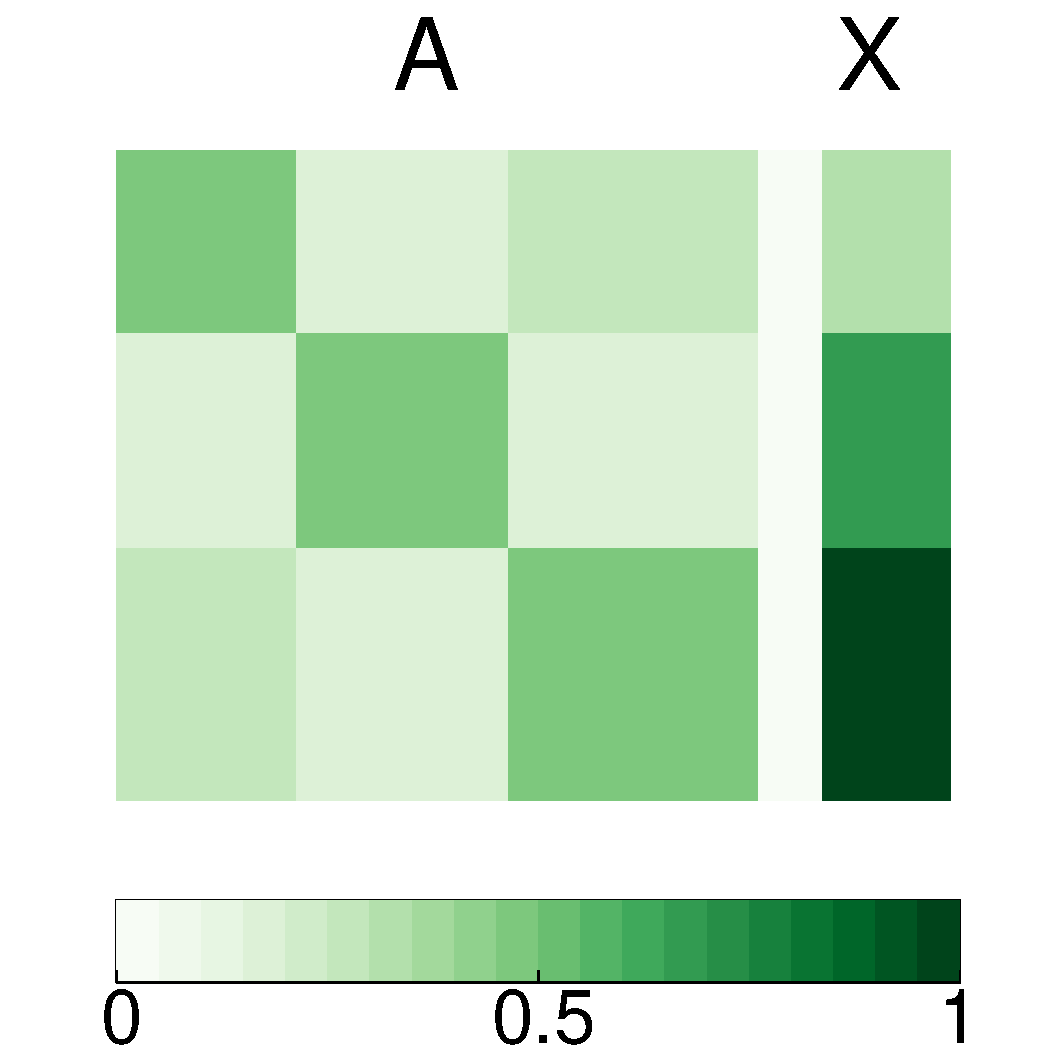
\includegraphics[width=\textwidth]{Pmat.pdf}
		\caption{}
		\label{fig:a}
	\end{subfigure}
	~ %add desired spacing between images, e. g. ~, \quad, \qquad, \hfill etc. 
	%(or a blank line to force the subfigure onto a new line)
	\begin{subfigure}[b]{0.23\textwidth}
		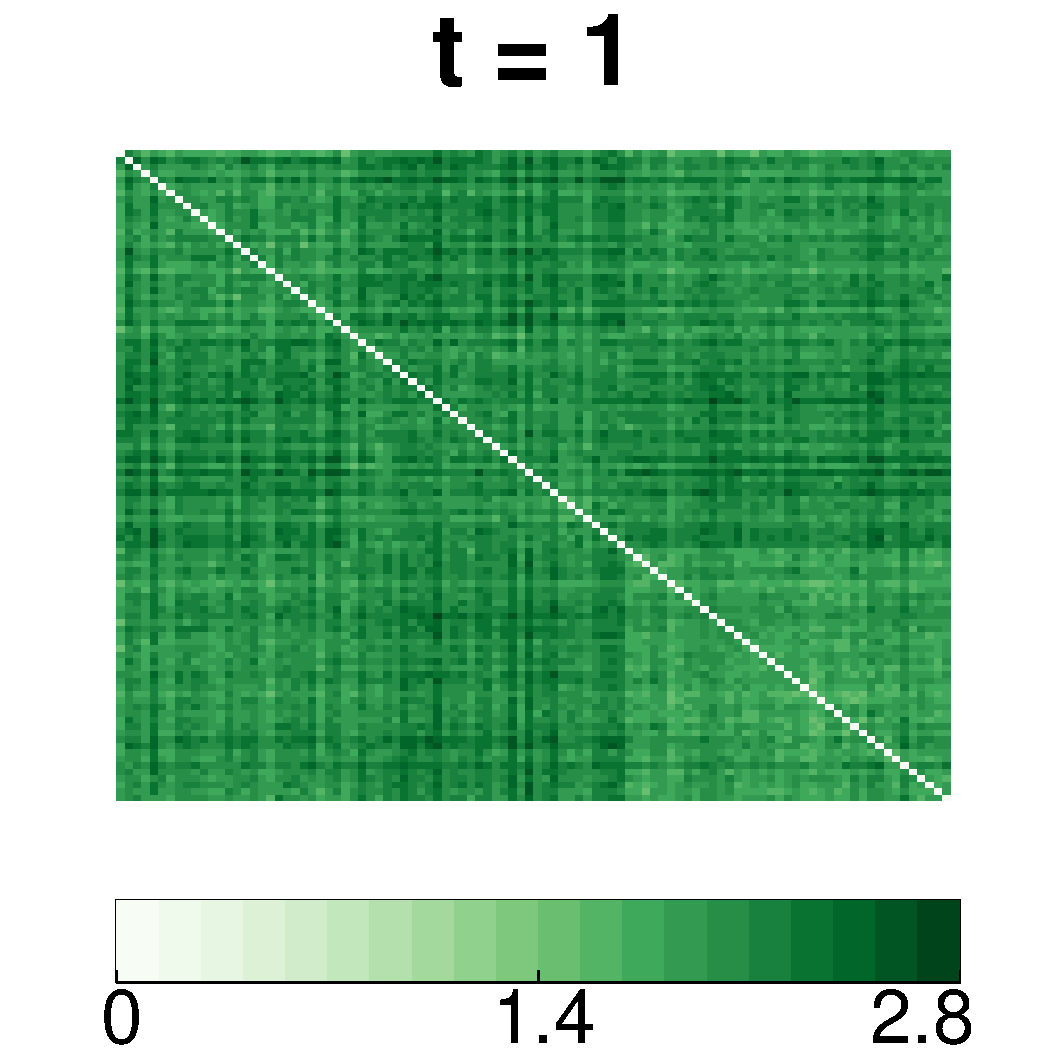
\includegraphics[width=\textwidth]{Dx1.pdf}
		\caption{}
		\label{fig:b}
	\end{subfigure}
	~ %add desired spacing between images, e. g. ~, \quad, \qquad, \hfill etc. 
	%(or a blank line to force the subfigure onto a new line)
	\begin{subfigure}[b]{0.23\textwidth}
		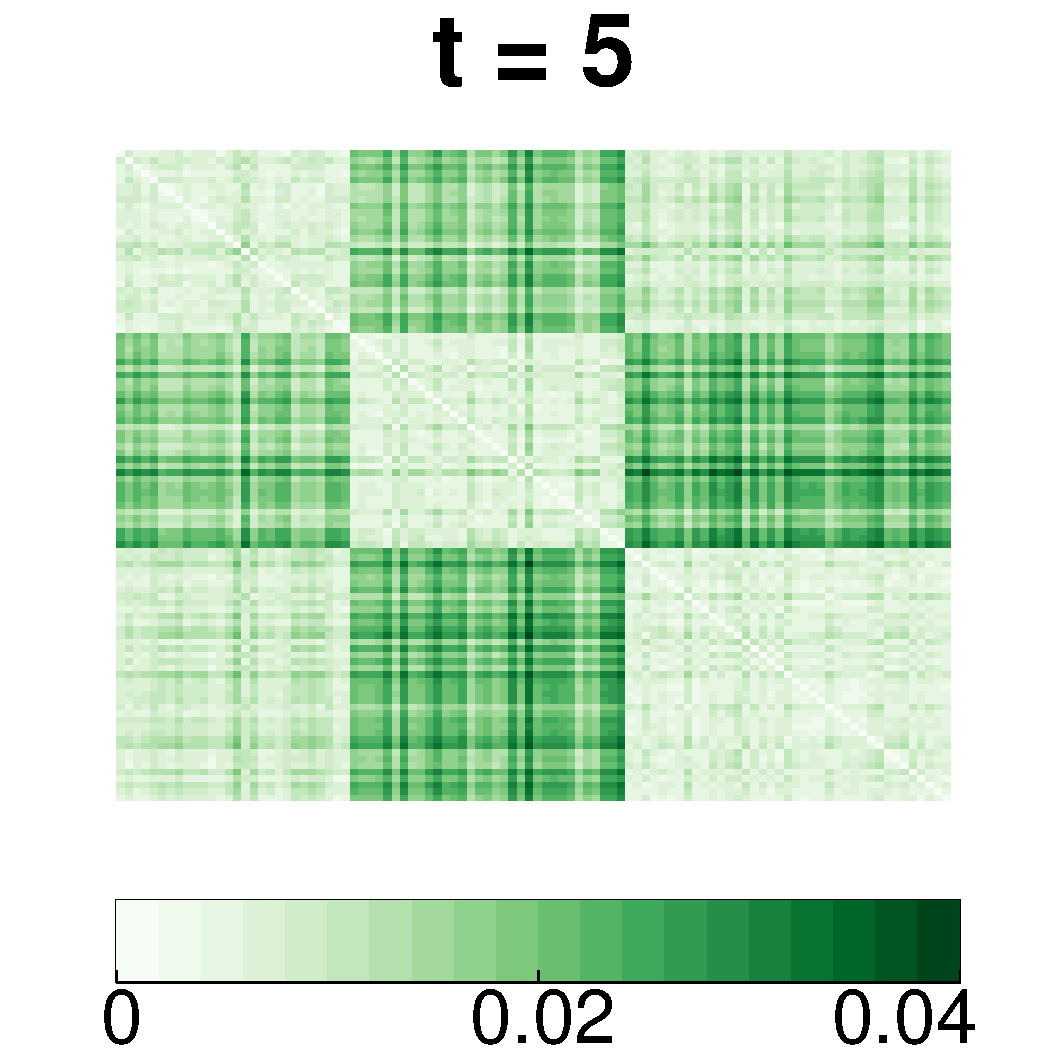
\includegraphics[width=\textwidth]{Dx5.pdf}
		\caption{}
		\label{fig:c}
	\end{subfigure}
	\begin{subfigure}[b]{0.23\textwidth}
		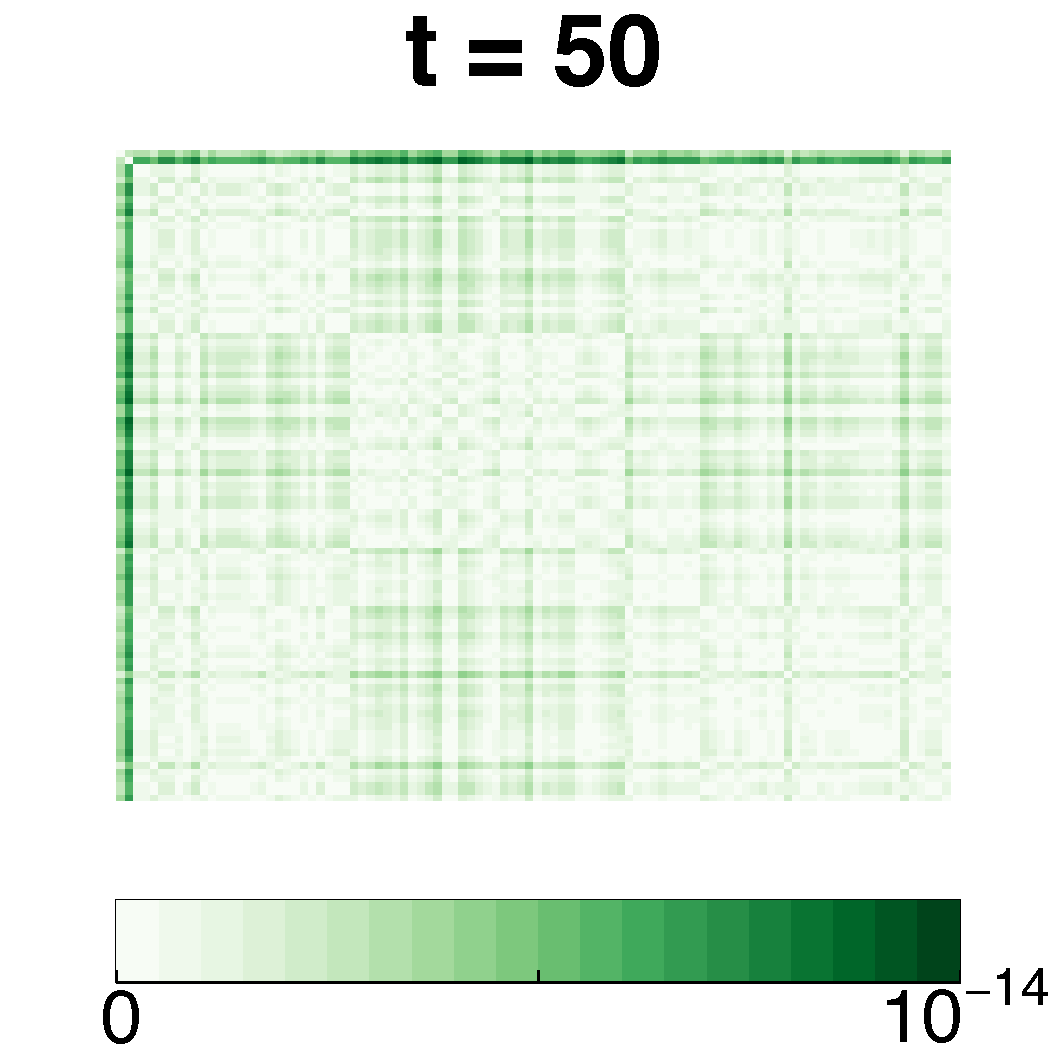
\includegraphics[width=\textwidth]{Dx50.pdf}
		\caption{}
		\label{fig:d}
	\end{subfigure}
	\caption{Panel (a) shows data generating probability of an adjacency matrix $\mathbf{A}$ and nodal attributes $\mathbf{X}$. Diffusion distances, as a proposed network metric, provide one-parameter family of network-based distances where as time goes by the pattern shown in the distance matrix changes, and at iteration time $t = 5$, distance distance in panel (c) illustrates most clear block structures and the most distinct dependency to the attributes $\mathbf{X}$.}
	\label{fig:diffusions}
\end{figure}

\vspace*{-0.4cm}
\subsection{Dependence Testing via \texttt{MGC}}
\label{ssec:method1}
The results in Section~\ref{ssec:method2} allow us to cast the network dependency test into the following framework: given sample data $(\mathbf{U}, \mathbf{X}) = \{  (\mathbf{u}_{i}, \mathbf{x}_{i} ) ; i = 1,2, \ldots, n \}$ that are identically distributed as $(\mathbf{u},\mathbf{x}) \in \mathbb{R}^{q \times q_x}$ ($q$ and $q_x$ are the respective feature dimension), we are looking to test whether their joint distribution equals the product of the marginals, i.e.,
\begin{align*}
& H_{0}: f_{\mathbf{u}\mathbf{x}}=f_{\mathbf{u}}f_{\mathbf{x}},\\
& H_{A}: f_{\mathbf{u}\mathbf{x}}\neq f_{\mathbf{u}}f_{\mathbf{x}}.
\end{align*}

If $(\mathbf{u}_{i}, \mathbf{x}_{i} )$ can be further assumed independently distributed for each $i$, we can directly use a wide range of consistent test statistics, including the distance correlation, the \texttt{HHG} test, and \texttt{MGC}. Take the distance correlation for example: denote $C_{ij} = \parallel \mathbf{u}_{i} - \mathbf{u}_{j} \parallel$ and $D_{ij} = \parallel \mathbf{x}_{i} - \mathbf{x}_{j} \parallel$ for $i,j=1,2, \ldots ,n$, where $\parallel \cdot \parallel$ is the Euclidean distance. The distance covariance is defined as 
\begin{equation}	 
\label{eq:dCov}
\texttt{dCov}(\mathbf{U}, \mathbf{X}) = \frac{1}{n^2} \sum\limits_{i,j=1}^{n} \tilde{C}_{ij} \tilde{D}_{ij},
\end{equation}
where $\tilde{C}$ and $\tilde{D}$ is doubly-centered $C$ and $D$ by its column mean and row mean respectively, i.e., $\tilde{C}=HCH$, where $H=I_{n}-\frac{J_{n}}{n}$ (the double centering matrix), $I_n$ is the $n \times n$ identity matrix (ones on the diagonal, zeros elsewhere), and $J_n$ is the $n \times n$ matrix of all ones. The distance correlation \texttt{dCorr} follows by normalizing the distance covariance and is in the range of $[0,1]$. The best property of distance correlation is its consistency against almost all alternatives, i.e., $\texttt{dCorr}(\mathbf{U}, \mathbf{X})$ has testing power $1$ for $n$ large, for any joint distributions of finite moment. The \texttt{MGC} test inherits the consistency of distance correlation, and significantly improves the finite-sample testing power via locating the optimal local correlation, i.e., excluding faraway distances in the computation of distance correlation.

However, as the \textit{i.i.d.} assumption is not satisfied under network topology, the consistency of distance correlation is no longer guaranteed when applied to arbitrary distance metric of the graph. In particular, neither the Euclidean distance of the adjacency vector nor the shortest-path distance can work together with distance correlation without breaking its consistency proof. 

Using Lemma~\ref{main_lemma}, our next result shows that both the \texttt{dCorr} and \texttt{MGC} defined on the diffusion distance can have the same consistency when extended to network dependency test of exchangeable graphs. This offers a principal approach to define correlations and testing dependency on network data. 

\begin{theorem}[\texttt{MGC} Consistency via Diffusion Distance]
Given an exchangeable graph $\mathbf{G}$ that is connected and unweighted, assume that $\mathbf{U} = \{ \mathbf{u}_{i} : i = 1,2, \ldots, n  \}$ is a diffusion map at any iteration time $t \in \mathbf{N}$ which is \textit{i.i.d.} as a random vector $\mathbf{u}$ of finite moment, conditioned on the underlying distribution; and the nodal attributes $\mathbf{X}=\{ \mathbf{x}_{i} :  i = 1,2, \ldots, n \}$ is \textit{i.i.d.} as a random vector $\mathbf{x}$ of finite moment 

Then for any $t$, $\texttt{dCorr}(\mathbf{U}, \mathbf{X}) \longrightarrow 0 \mbox{ as } n \rightarrow \infty$ if and only if $\mathbf{u}$ is independent of $\mathbf{x}$. Therefore, both \texttt{dCorr} and \texttt{MGC} are consistent for testing dependence between $\mathbf{u}$ and $\mathbf{x}$.
	\label{theoremMain}
\end{theorem}
The proof is postponed to the Appendix.

%Note that if $\{ \mathbf{w}_{i} : i = 1,2,\ldots, n \}$ are \textit{i.i.d}, they are also exchangeable. Thus estimated latent network factors, which are assumed \textit{i.i.d} by \cite{fosdick2015testing} can also be applied to Theorem~\ref{theoremMain}. We already have shown that even under undirected network, diffusion maps remain exchangeable at each diffusion time point $t$. 

%%%%%%%%%%%%%%%%%%%%%%%%%%%%%%%%%%%%%%%%%%%%%%%%%%
\section{Simulation Study}
\label{sec:simulation}
	\vspace*{-0.2cm}
Next we investigate our approach via simulated models and empirical performances. In the simulation studies, we compare the empirical testing powers of four test statistics: \texttt{MGC}, \texttt{dCorr}, \texttt{HHG}, and the likelihood ratio test by Fosdick and Hoff (\texttt{FH})~\cite{fosdick2015testing}. For the first three statistics, we further consider three different metrics of the network topology: the Euclidean distances of the diffusion maps at $t=5$ (\texttt{DM}), of each column of adjacency matrix (\texttt{AM}), and of the latent factors (\texttt{LF}, which is based on singular value decomposition of the adjacency matrix). The \texttt{FH} likelihood ratio test must always be based on the latent factors.

For each simulation model and each test, we repeatedly generate sample data for $500$ times, carry out the permutation test, and reject the null if the resulting p-value is less than $0.05$. The testing power of each method equals the percentage of correct rejection. We will mainly consider the stochastic block model (SBM) and its degree-corrected version for the simulation models, which are often used in community detection. 

Let us first consider SBM with $3$ blocks, i.e., partition the nodes into $3$ communities, and generate the edges by a Bernoulli random variable whose probability that is determined by the communities of the connecting nodes. Assume $n=100$ nodes whose class label $\mathbf{x}_i$ takes values in $0,1,2$ equally likely. The edge probability is designed as
\begin{equation}
\label{eq:Three}
E(A_{ij} | X_{i}, X_{j}) = 0.5 I(|X_{i} - X_{j}| = 0) + 0.2 I(|X_{i} - X_{j}| = 1) + 0.3 I(|X_{i} - X_{j}| = 2), \quad i,j = 1, \ldots, n = 100.
\end{equation} 
Namely, within-block edge probability is $0.5$, between-block edge probability is $0.2$ or $0.3$ depending on the communities. This 3-block model describes a nonlinear dependency between the network topology and the class labels, where \texttt{MGC} should work the best when coupled with a proper metric. Indeed, Figure~\ref{fig:threeSBM} illustrates that \texttt{MGC} combined with diffusion maps yields the most superior power comparing to all other benchmarks.

\begin{SCfigure}[][ht]
	\centering
	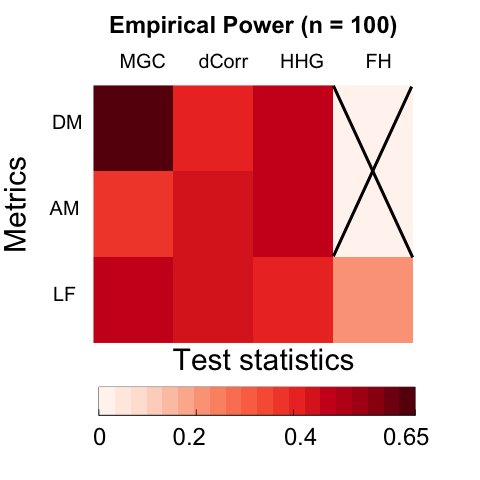
\includegraphics[width=0.4\paperwidth, height=0.4\paperwidth]{ThreeSBM_results_short.png}
	\caption{The power heatmap in SBM with three blocks, for all possible combinations of test statistics with distance metrics. \texttt{MGC} with the diffusion maps yields the best power comparing to all other methods. }
	\label{fig:threeSBM}
\end{SCfigure}

To further understand the advantage of \texttt{MGC}, next we fix the distance as the diffusion distance, and control the amount of \textit{nonlinear dependency} through changing the value of $\theta \in (0, 1)$ in the edge probability:
\begin{equation}
E(A_{ij} | X_{i}, X_{j}) = 0.5 I(|X_{i} - X_{j}| = 0) + 0.2 I(|X_{i} - X_{j}| = 1) + \theta I(|X_{i} - X_{j}| = 2), \quad i,j = 1, \ldots, n = 100.
\label{eq:mono}
\vspace*{-0.4cm}
\end{equation}
When $\theta > 0.2$, the network dependency changes from a close to linear relationship to strongly nonlinear. Figure~\ref{fig:powerplot} shows the testing power with respect to increasing $\theta$, and there is a clear trend that both the \texttt{dCorr} and \texttt{FH} tests have deteriorating power while \texttt{MGC} is very stable against varying $\theta$. The same phenomenon holds by varying other edge probabilities. Therefore, the \texttt{MGC} capability to better capture the nonlinear dependencies shown in \cite{shen2016discovering} carries over to network dependence testing.
\begin{figure}[ht]
	\centering
	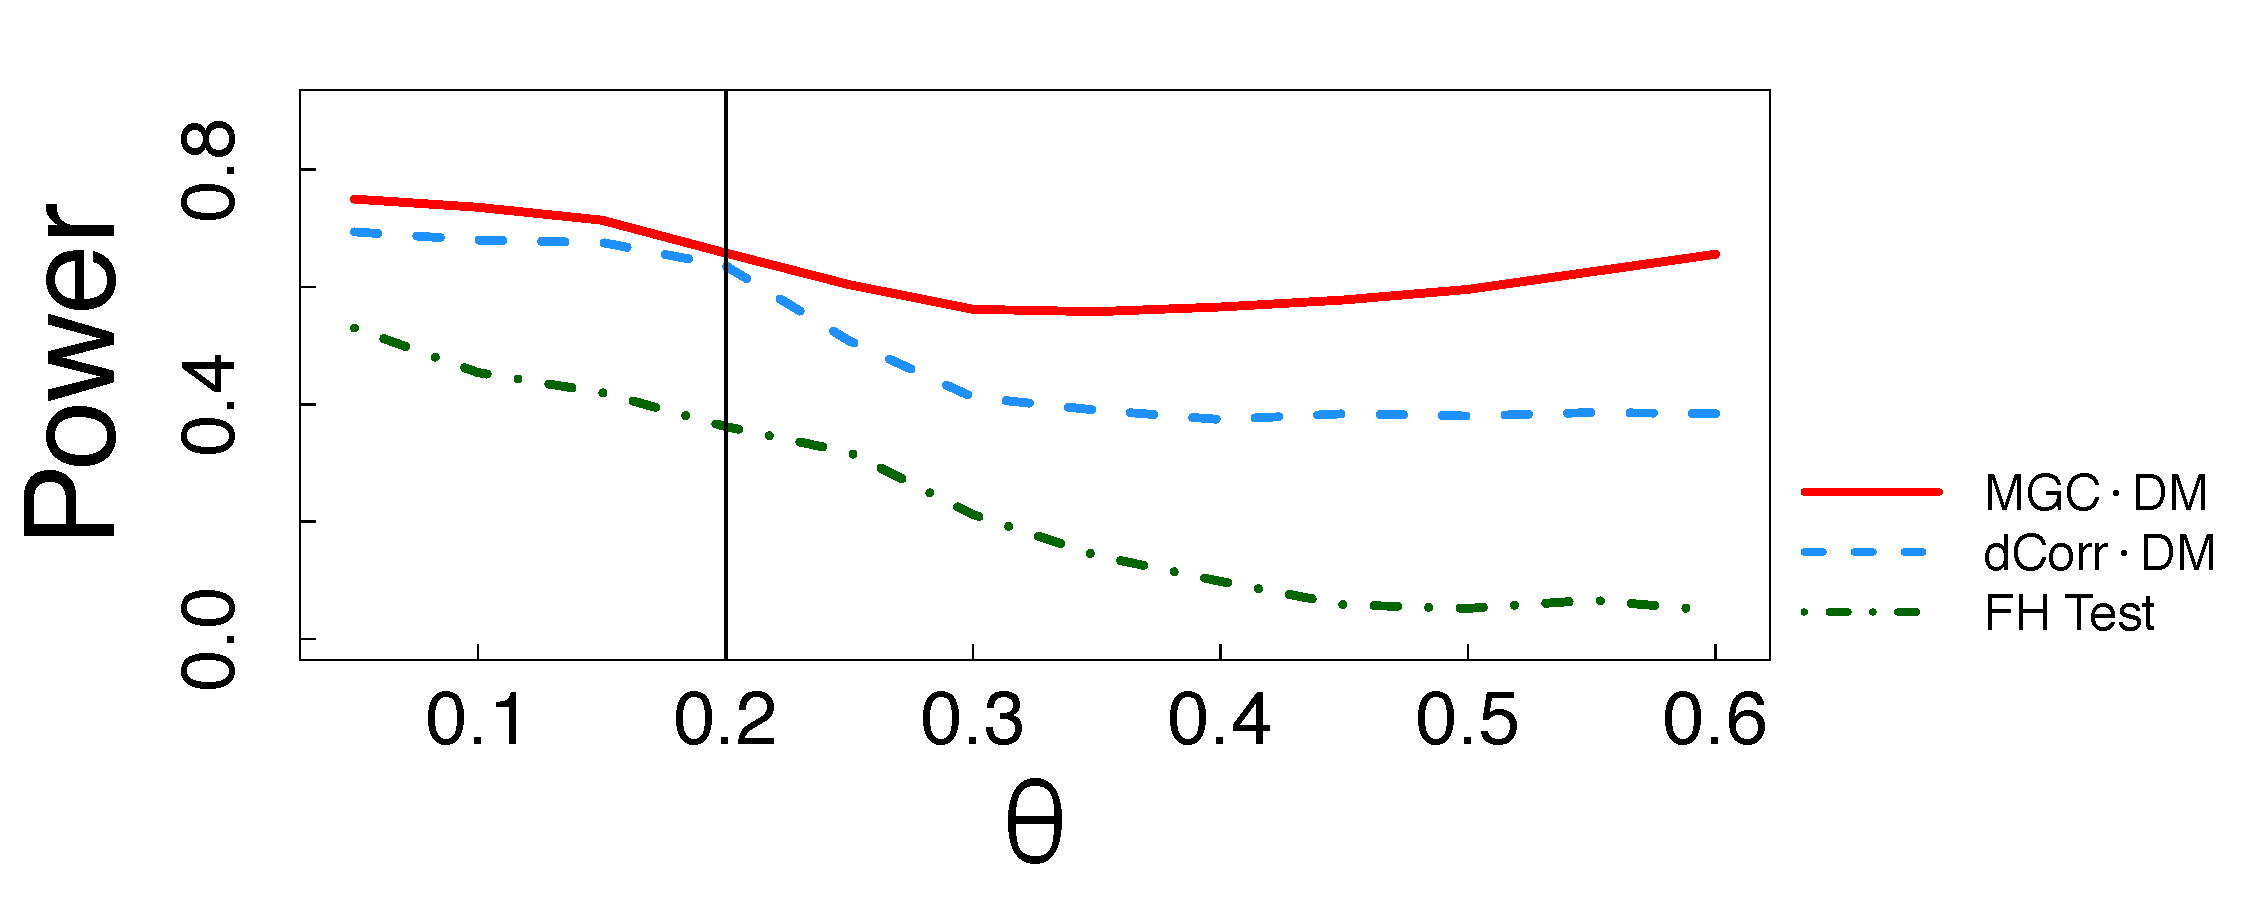
\includegraphics[width=0.7\linewidth]{mono_short.pdf}
	\caption{The power curve with respect to increasing $\theta$ in SBM with three blocks, for \texttt{MGC}, \texttt{dCorr}, and \texttt{FH}. Larger $\theta$ implies stronger nonlinear dependency, while $\theta<0.2$ has close-to-linear dependency. \texttt{MGC} is the best performing method throughout all possible $\theta$.}
	\label{fig:powerplot}
\end{figure}

% degree-corrected two block model
Our next simulation is based on the degree-corrected stochastic block model (DCSBM) with two blocks. This time we fix the test statistic to \texttt{MGC}, but varying the distance metrics. DCSBM adds another random variable $V_{i}$ associated with each node to vary the node degrees, which is a generalization of the stochastic block model and provides a better fit to real networks. Setting $n=250$, suppose that the nodal attributes / class label $X_i$ takes values in $0$ and $1$ equally likely and the edge probabilities are specified by 
\vspace*{-0.4cm}
\begin{equation}
E( A_{ij} | \mathbf{X}, \mathbf{V} )  = 0.2 V_{i} V_{j} \cdot I ( |X_{i} - X_{j}| = 0 ) + 0.05 V_{i} V_{j} \cdot I(|X_{i} - X_{j}| = 1),
\label{eq:tau}
\vspace*{-0.4cm}
\end{equation} 
where $V_{i} \overset{i.i.d}{\sim} Uniform(1 - \tau, 1 + \tau)$ for $i = 1, \ldots, n$, and $\tau$ is a parameter to control the amount of variability of the edge distribution. Figure~\ref{fig:dcSBM} shows the testing power based on the above model with respect to different metrics, and the diffusion distance is clearly the most superior one regardless of $\tau$.

\begin{figure}[ht]
	\centering
	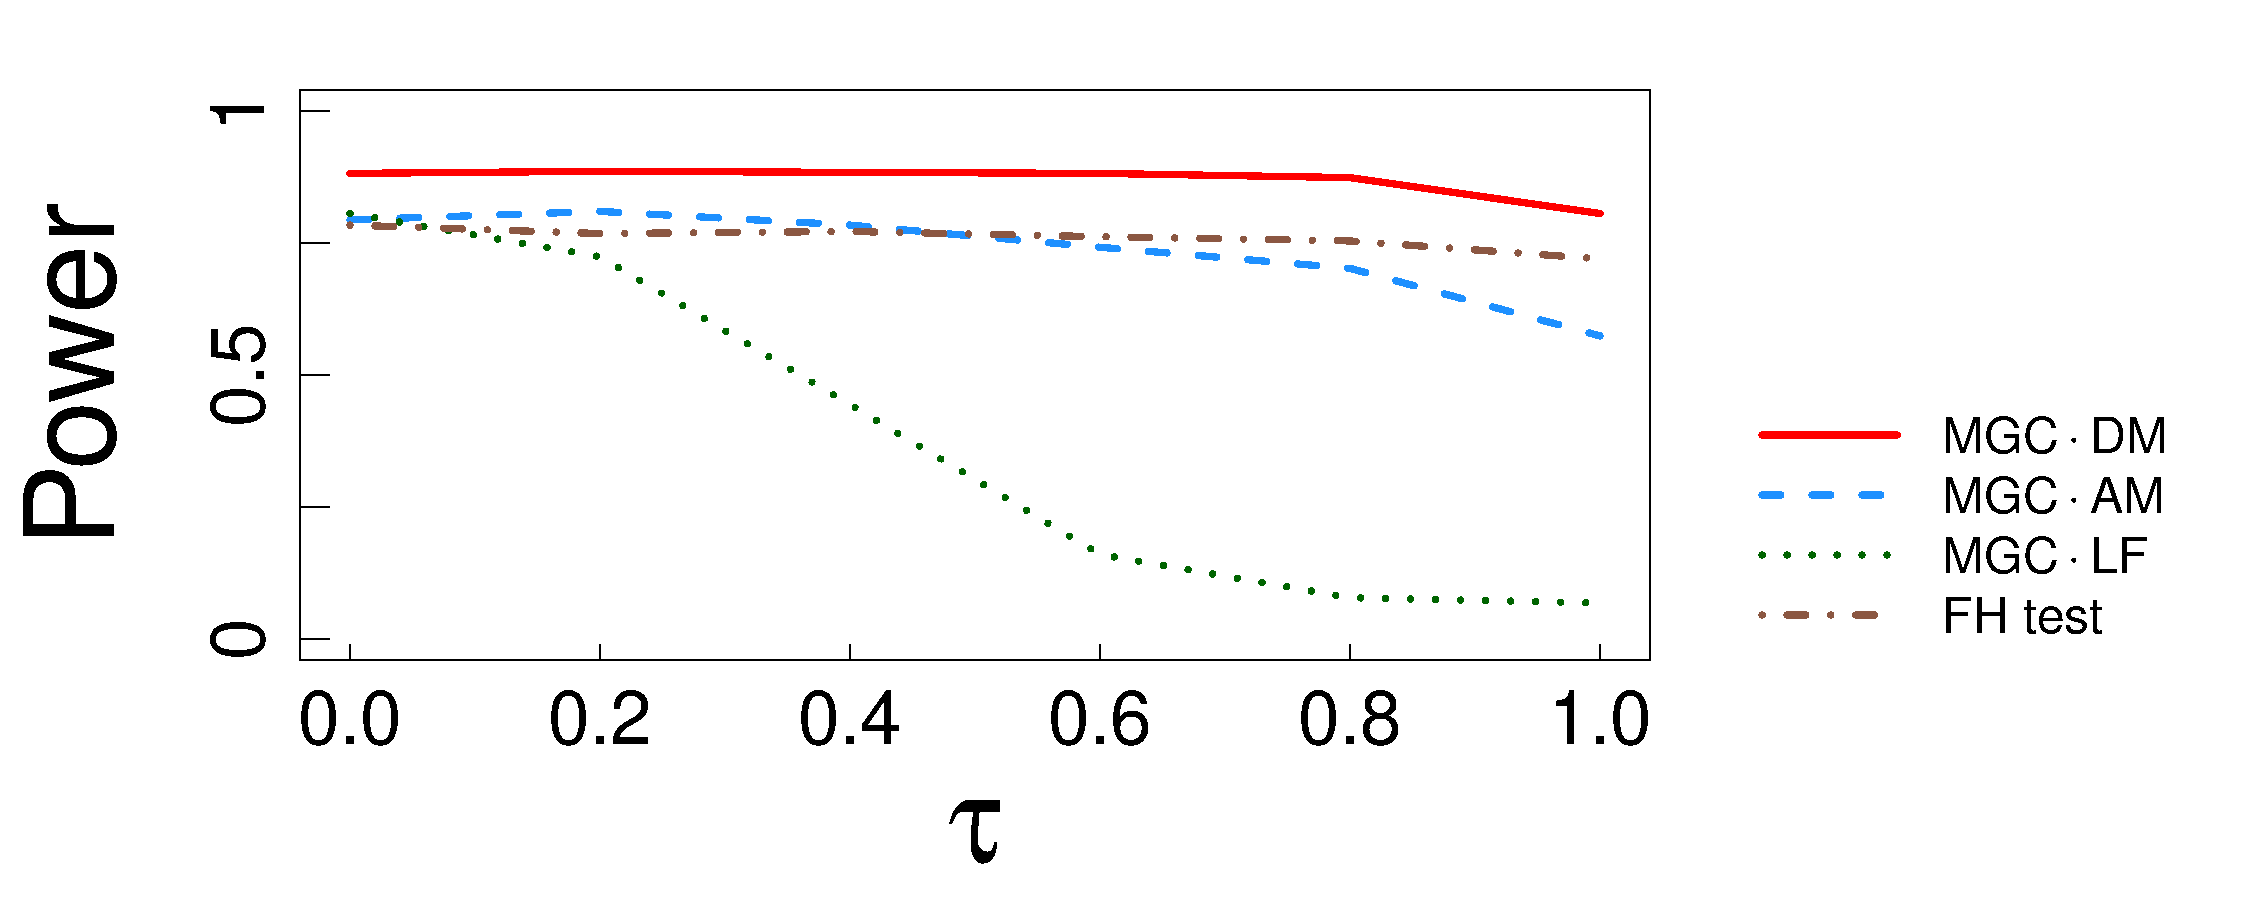
\includegraphics[width=0.7\linewidth]{tau_short.pdf}
	\caption{The power curve with respect to increasing $\tau$ in DCSBM with two blocks, for \texttt{MGC} with different distance metrics and \texttt{FH}. The diffusion distance exhibits the best testing power comparing to other metrics, and is better than the \texttt{FH} test.}
	\label{fig:dcSBM}
	\vspace*{-0.5cm}
\end{figure}

%%%%%%%%%%%%%%%%%%%%%%%%%%%%%%%%%%%%%%%%%
%\section{Real Data Examples}
%\label{sec:real}
%\begin{figure}[ht]
%	\centering
	%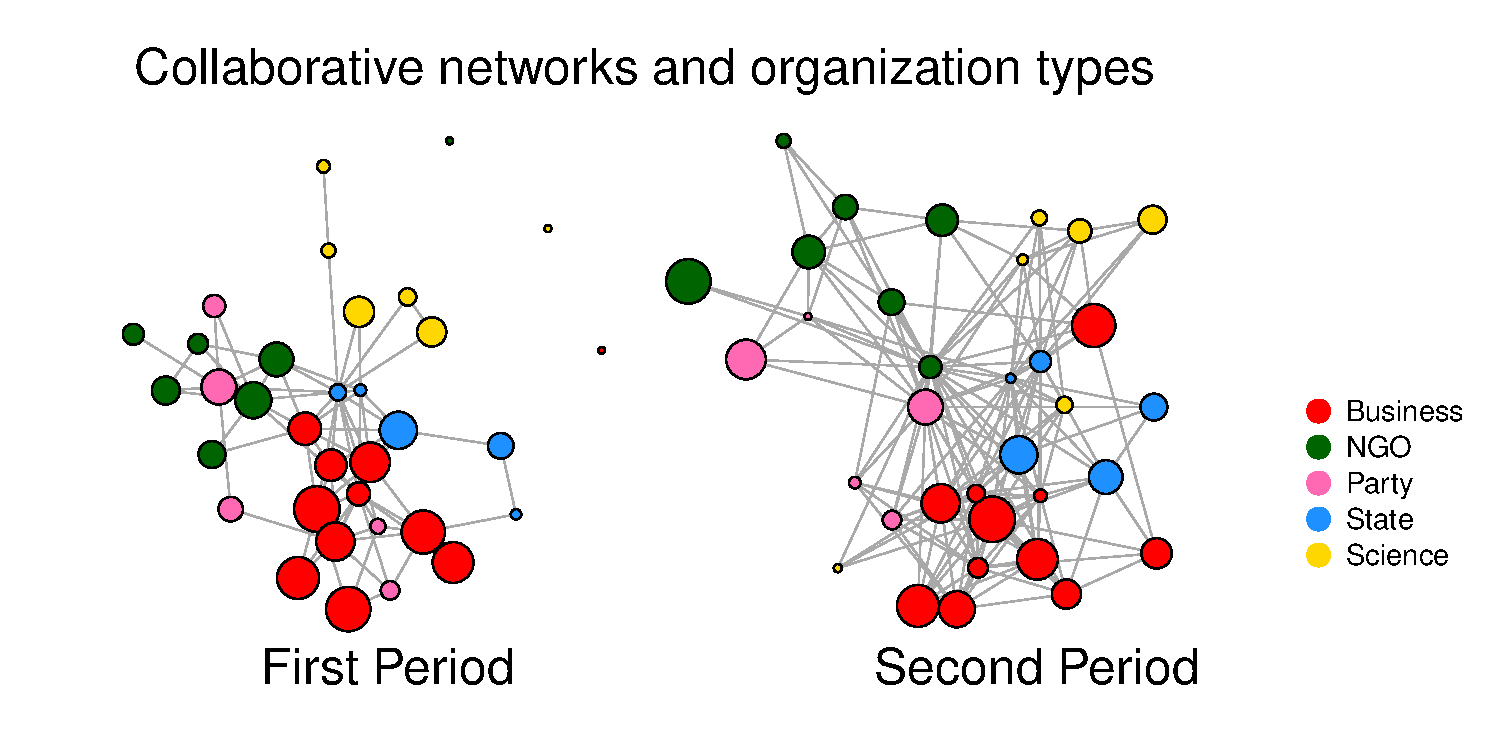
\includegraphics[width=\linewidth]{../Figure/two_politics.pdf}
	%\caption{Both panels depict the collaborative networks during the two time periods having significant network dependency in types of organizations. Using \texttt{MGC} statistics, we are not only able to test network independence but also calculate each node's amount of contribution to detecting dependence, which is proportional to node size here. You can tell that the tendency to collaborate within the same type is strongest among the business group while scientist relatively collaborates less with any others, especially in the first period.}
	%\label{fig:politics}
%\end{figure}
%In the field of political science, who exerts more powerful impacts than the others over political network and which factors impact on the power differentials are one of the interests~\cite{ingold2014structural}. \cite{minhas2016inferential} made an inference from political networks~\cite{cranmer2016navigating} via the additive and multiplicative effects (AME). The AME model estimates the latent factors and uses them to test independence with the nodal attributes. Among diverse attributes that \cite{cranmer2016navigating} provided, we focus on the types of organizations and how 34 political organizations having different types are participating policy network. We changed a given directed network into undirected network and use a dissimilarity matrix for distance matrix of the attributes, i.e., $\parallel \mathbf{X}_{i}  - \mathbf{X}_{j} \parallel = 0$ if and only if node $i$ and node $j$ are from the same type and one otherwise. Two collaboration networks comprised of the same set of nodes across two time periods are provided~\cite{ingold2014structural}. Figure~\ref{fig:politics} and Figure~\ref{fig:barplots} illustrates these two networks and shows each node's reliance on its organization type when collaborating. During the two periods, the network independence test statistics of \texttt{MGC} (p-value : (0.002 , 0.002)) and \texttt{dCorr} (p-value : ( 0.000, 0.000)) using diffusion distance matrices result in significant p-values across diffusion times from $t=1$ to $t=10$. The conclusion from the \texttt{FH} test (p-value : ( 0.000, 0.000)) is also the same.  
%\begin{figure}[ht]
	%\centering
	%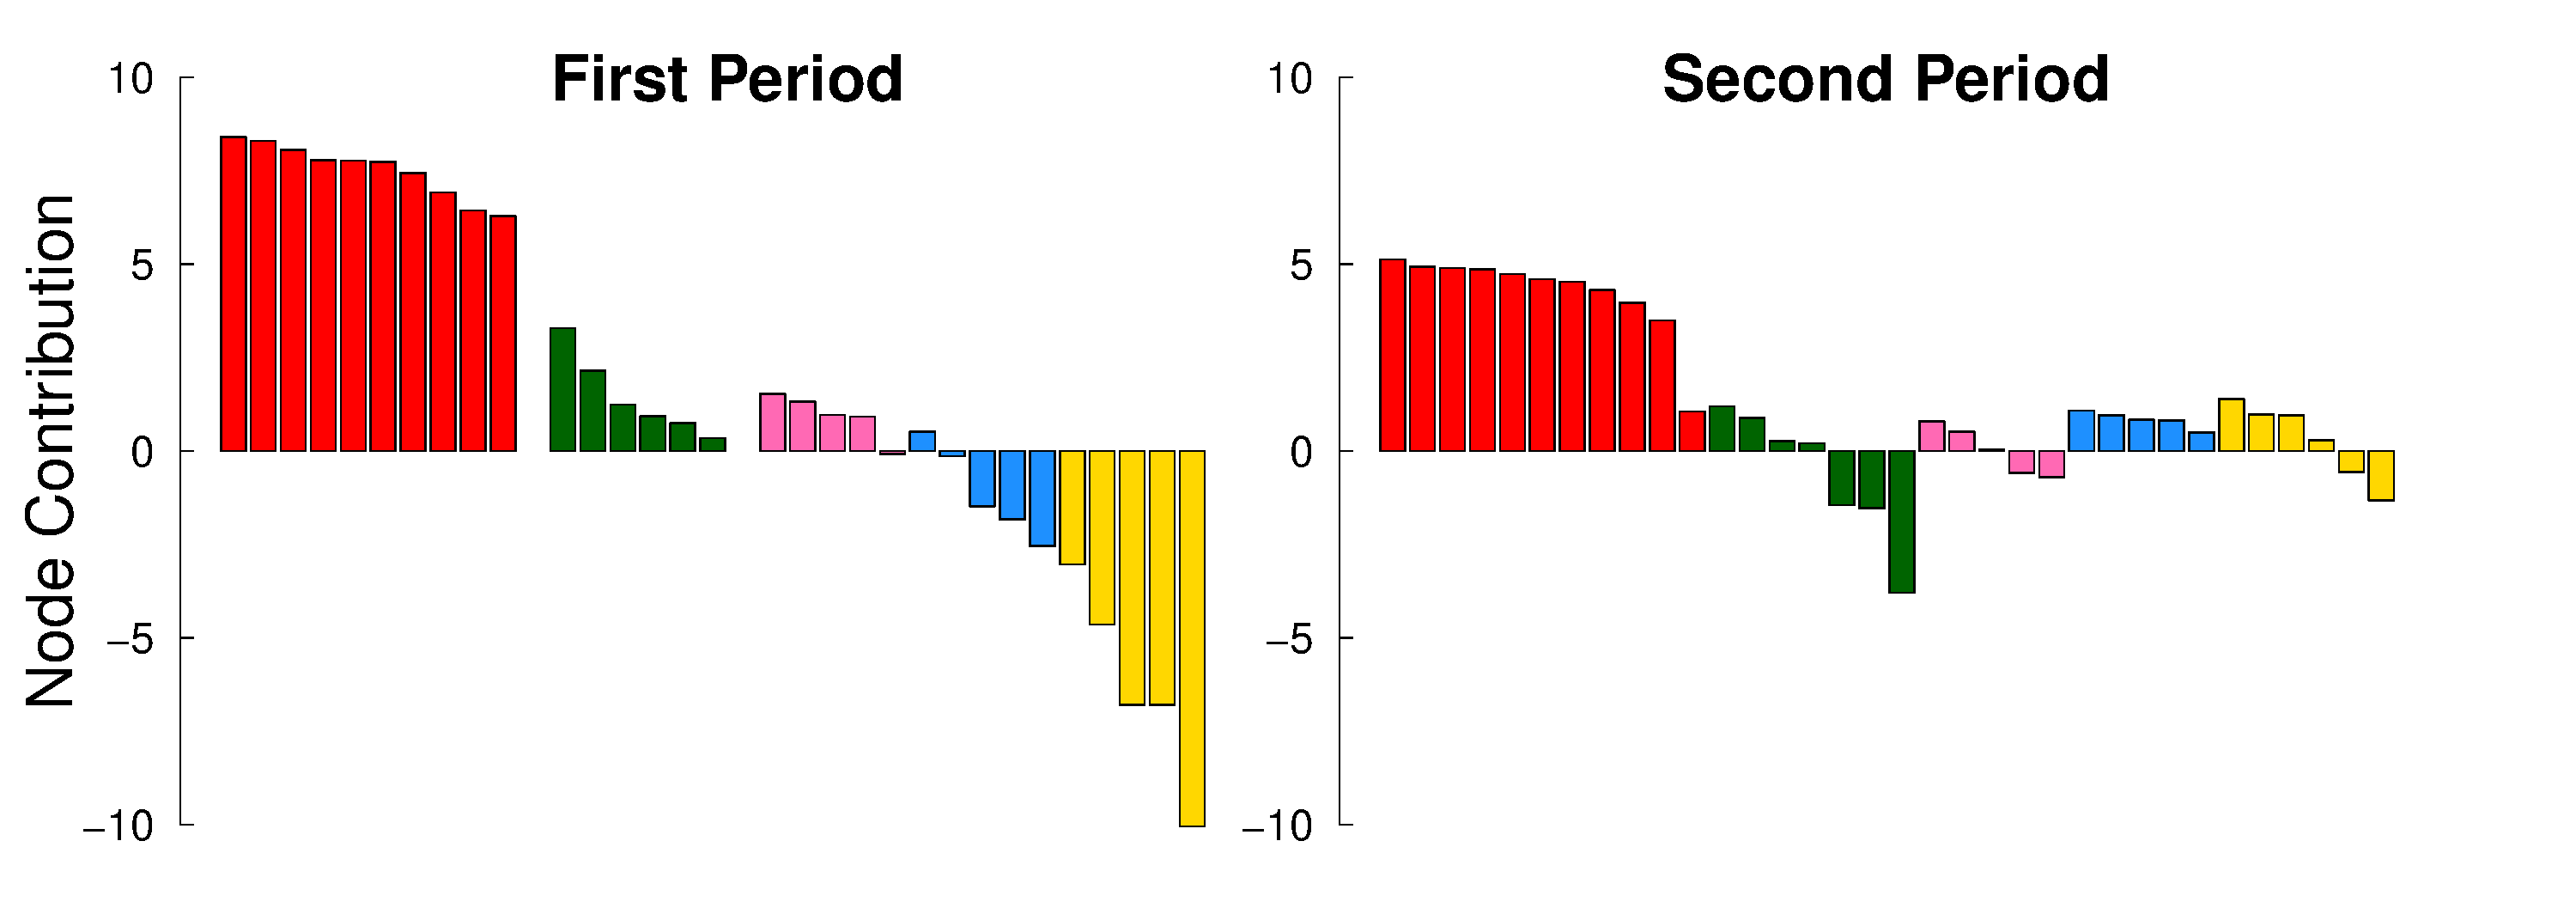
\includegraphics[width=\linewidth]{../Figure/barplots_nolegend.pdf}	
	%\caption{In the first period, we have two extreme cases among the business group and science group, which reflects our observations in Figure~\ref{fig:politics}. Generally organizations cooperate more actively between different types in the second period but still their collaboration network is highly dependent on their organization types especially for business group.}
	%\label{fig:barplots}
%\end{figure}


%%%%%%%%%%%%%%%%%%%%%%%%%%%%%%%%%%%%%%%%
\vspace*{-0.5cm}
\section{Conclusion And Future Work}
\label{sec:conc}
	\vspace*{-0.2cm}
In this paper, we combined recent progress in dependency testing and metric learning into the graph domain, and showed that \texttt{MGC} on the diffusion distance offers an elegant and powerful solution to the network dependency problem. We proved that this method is consistent under most popular graph models; and empirically demonstrated its superior power comparing to using other distance metrics, or other correlation measures and tests.

There are a number of additional potential extensions of this work. First, how to choose a better diffusion time $t$, or find a $t$ with provable finite-sample performance, may provide further insight into and establish a more solid foundation of this approach. Second, the network dependence testing here is actually equivalent to the two-sample test, i.e., whether two graphs come from the same distribution; thus our approach readily offers a new nonparametric two-sample test on networks, for which more investigation will bring a valuable addition to the graph analysis. Third, with a few alterations, the new correlation measure on graph may be utilized for other tasks, such as feature screening, outlier detections, clustering, and classification, etc.

%convince that \texttt{MGC}, merged with a family of diffusion distance, provides us powerful independence test statistics in network. Having multiscale statistics, i.e.~one parameter family of statistics, is not avoidable because we regard distance between the nodes over network as a dynamic process. Through simulation studies, we demonstrate that our methods perform better than the others especially under nonlinear dependency, and we are able to measure each node's contribution to detecting dependency. Deriving the contributions is particularly important when there have possibly different amounts of the dependencies among the nodes.  

%However obtaining a full family of statistics are computationally infeasible. Also we did not suggest any theoretically supported tools to select one metrics among them so thus we have one single statistic. As an ad hoc, we selected an \textit{optimal} diffusion time $t$ with highest power from $t=1$ to $t=10$ for our simulation since we could observe a stabilized empirical power within this period. Developing the adaptive method to find this optimal $t$ where dependence is maximized would be a natural next step. Despite these shortcomings, we expect that we could also enjoy the properties of \texttt{MGC} and a family of diffusion distances in solving diverse problems which require to utilize local relationship of the data sets. For instance, we might be able to implement independence testing between two networks of same size by using diffusion distance of each network to investigate whether a pair of networks are topologically or structurally independent. This kind of work would shed light on revealing any relationship between the data sets which are not necessarily a random vector.

%%%%%%%%%%%%%%%%%%%%%%%%%%%%%%%%%%%%%%%%%%%%
\vspace*{-0.5cm}
\bibliography{reference}
%\bibliographystyle{plainnat}
%%%%%%%%%%%%%%%%%%%%%%%%%%%%%%%%%%%%%%%%%%%%%%
\vspace*{-0.5cm}
\section{Appendix}
\vspace*{-0.2cm}
\subsection{Lemmas and Theorems}
\label{ssec:proof}

%%%%%%%%%%%%%%%%%%%%%%%%%%%%%%%%%%%%%%%%	
\begin{proof}[\textbf{Proof of Lemma~\ref{main_lemma}}]
	Diffusion map at time $t$ is represented as follows :
	\begin{equation}
	\mathbf{U}_{t}(i) = \begin{pmatrix} \lambda^{t}_{1} \phi_{1}(i) & \lambda^{t}_{2} \phi_{2} (i)  & \cdots & \lambda^{t}_{q} \phi_{q}(i) \end{pmatrix} \in \mathbb{R}^{q},
	\end{equation}
where $\{ \lambda_{j} \}$ and $\{ \phi_{j}  \}$ are the non-zero eigenvalues and corresponding eigenvectors of the transition matrix $\mathbf{P}$. Therefore to guarantee the exchangeability of $\mathbf{U}_{t}$, it suffices to show the exchangeability of $\mathbf{P}$.
	
Assume that $\mathbf{G}$ is an connected and unweighted exchangeable graph, i.e., $(A_{ij}) \stackrel{d}{=} \big( A_{\sigma(i) \sigma(j)} \big)$. Since $A_{ij}$ is binary, $A_{ij} / \sum\limits_{j} A_{ij} = A_{ij} /  (1 + \sum\limits_{l \neq j} A_{il})$. Moreover, $A_{ij}$ and $(1 + \sum\limits_{l \neq j} A_{il})$ are conditionally independent according to \textit{Aldous-Hoover Theorem} \cite{aldous1981representations}, and $A_{\sigma(i) \sigma(j)}$ and $(1 + \sum\limits_{l \neq j} A_{\sigma(i) \sigma(l)})$ are also conditionally independent. Then the following joint exchangeability of transition probability holds for $i \neq j, i,j = 1,2, \ldots,n$:	
	\begin{equation}
		\vspace*{-0.2cm}
	\big( P_{ij} \big) = \left(  \frac{A_{ij}}{1 - A_{ij} + \sum\limits_{j=1}^{n} A_{ij} } \right)  \stackrel{d}{=} \left( \frac{A_{\sigma(i) \sigma(j)} }{1 - A_{\sigma(i) \sigma(j)} + \sum\limits_{\sigma(j) = 1}^{n} A_{\sigma(i) \sigma(j)} } \right) = \big( P_{\sigma(i) \sigma(j)} \big).
	\end{equation}
When $i = j$, $P_{ij} = P_{\sigma(i) \sigma(j)} = 0$ for $i=1,2, \ldots, n$. Thus, transition probability is also exchangeable. This results exchangeable eigenfunctions $\{ \Phi(1), \Phi(2), , ... , \Phi(n) \}$ where $\Phi(i) := \begin{pmatrix} \phi_{1}(i) & \phi_{2}(i) & \cdots & \phi_{q}(i) \end{pmatrix}^{T}$, $i=1,2, \ldots, n$. Thus diffusion maps at fixed $t$, $\mathbf{U}_{t} = \begin{pmatrix} \Lambda^{t} \Phi(1)  & \Lambda^{t} \Phi(2) & \cdots & \Lambda^{t} \Phi(n)  \end{pmatrix}$ are exchangeable. Furthermore by \textit{de Finetti's Theorem}~\cite{diaconis1980finite}, we can say that $\mathbf{U}_{t} = \{ \mathbf{U}_{t}(1), \mathbf{U}_{t}(2), \ldots, \mathbf{U}_{t}(n)  \}$ are independent conditioned on their underlying distribution.
\end{proof}

%%%%%%%%%%%%%%%%%%%%%%%%
\begin{proof}[\textbf{Proof of Theorem~\ref{theoremMain}} Consistency of \texttt{dCorr} applied to exchangeable variables]

Assume that an exchangeable sequence of $(\mathbf{U}, \mathbf{X}) = \{ (\mathbf{u}_{i}, \mathbf{x}_{i}) ; i = 1,2, \ldots, n \}$ is identically distributed as $(\mathbf{u}, \mathbf{x})$ with finite second moment. Then we have 
\begin{eqnarray}
\mathcal{V}_{n}^{2}(\mathbf{U},\mathbf{X}) &\longrightarrow \mathcal{V}^{2}(\mathbf{u},\mathbf{x}) \quad \quad \mbox{ as } n \rightarrow \infty
\label{eq:conv1}
\end{eqnarray}
where $\mathcal{V}^{2} (\mathbf{u},\mathbf{x}) := \| g_{\mathbf{u},\mathbf{x}}(t,s) - g_{\mathbf{u}}(t) g_{\mathbf{x}}(s) \|^2$, and $g_{\cdot}$ is a characteristic function, e.g., $g_{\mathbf{u},\mathbf{x}}(t,s) = E\{\exp\{i \left\langle t,\mathbf{u} \right\rangle  +i \left\langle  s,\mathbf{x}\right\rangle \}\}$. This follows exactly the same as \textit{Theorem 1} in \cite{szekely2007measuring}. Note that this Lemma always holds without any assumption on $\{(\mathbf{u}_{i},\mathbf{x}_{i}), i=1,2,...,n\}$.

Followed by \textit{de Finetti's Theorem}, if and only if $\{ \mathbf{u}_{i} \}$ are (infinitely) exchangeable, there exists an underlying distribution $f_{\mathbf{u}}$ of $\mathbf{u}$ such that $\mathbf{u}_{i}  \overset{i.i.d}{\sim} f_{\mathbf{u}}, i = 1, \ldots, n$. By the same logic, we have an underlying distribution $f_{\mathbf{x}}$ where $\mathbf{x}_{i} \overset{i.i.d}{\sim} f_{\mathbf{x}}$. Then under the assumption of finite second moment of the underlying distributions and measurable, conditioned random functions, we have a strong large number for V-statistics followed by \cite{szekely2007measuring}, i.e., 
\begin{eqnarray}
\displaystyle\int_{D(\delta)}{\|g_{\mathbf{u},\mathbf{x}}^{n}(t,s)-g_{\mathbf{u}}^{n}(t)g_{\mathbf{x}}^{n}(s)\|^{2}}dh &\stackrel{n \rightarrow \infty}{\longrightarrow} 
\displaystyle\int_{D(\delta)}{\|g_{\mathbf{u},\mathbf{x}}(t,s)-g_{\mathbf{u}}(t)g_{\mathbf{x}}(s)\|^{2}}dh,
\label{eq:SLLN}
\end{eqnarray}
where $D(\delta)=\{(t,s):\delta \leq |t|_{p} \leq 1/\delta,\delta \leq |s|_{q} \leq 1/\delta\}$, and $h(t,s)$ is the weight function chosen in \cite{szekely2007measuring}. 	
It follows that 
\begin{eqnarray}
\mathcal{V}_{n}^{2}(\mathbf{U},\mathbf{X}) &\rightarrow 0 \quad \mbox{ as } n \rightarrow \infty
\label{eq:conv2}
\end{eqnarray}
if and only if $g_{\mathbf{u},\mathbf{x}}(t,s) = g_{\mathbf{u}}(t) g_{\mathbf{x}}(s)$, i.e., $\mathbf{u}$ is independent of $\mathbf{x}.$ Therefore, the \texttt{dCorr} converges to $0$ if and only if $\mathbf{u}$ and $\mathbf{x}$ are independent; and its testing power converges to $1$ under any joint distribution of finite moments. Since the multiscale generalized correlation based on any consistent global correlation is also consistent~\cite{shen2016discovering}, \texttt{MGC} statistic constructed by \texttt{dCorr} or \texttt{mCorr} is also consistent in testing dependence.
\end{proof}
%%%%%%%%%%%%%%%%%%%%%%%%%%5
%\begin{proof}[\textbf{Proof of Theorem~\ref{theorem2}} Consistency of \texttt{MGC} applied to exchangeable variables]
	
%Under the exchangeability and finite second moment assumptions of underlying distribution, $\mathcal{V}^{2}_{n}(\mathbf{W},\mathbf{Y}) \xrightarrow{n \rightarrow \infty}  0$ if and only if underlying distribution of $\{\mathbf{w}_{i} \}$, $f_{\mathbf{w}}$ is independent from underlying distribution of $\{ \mathbf{y}_{i}  \}$, $f_{\mathbf{y}}$. Now suppose that we have undirected, connected network $\mathbf{G}$ with a family of diffusion maps $\{ \mathbf{u}_{t}  \}$ and with nodal attributes $\{ \mathbf{x}  \}$. We have shown in the Lemma~\ref{main_lemma} that $\{ \mathbf{u}_{t}  \}$ are exchangeable for each $t \in \mathbb{N}$. Thus there exists an underlying distribution of $\mathbf{u}_{t}$ such that $\mathbf{u}_{t}(i) \overset{i.i.d}{\sim} f_{\mathbf{u}^{(t)}}$ for each of $t= 1,2,\ldots $; and we have $\mathbf{x}_{i} \overset{i.i.d}{\sim} f_{\mathbf{X}}$. Under the assumption of finite second moment of $\mathbf{u}^{(t)}$ and $\mathbf{x}$, \texttt{MGC} statistics constructed by $\{  (  \mathbf{u}_{t}(i), \mathbf{x}_{i} ) : i = 1,2,\ldots, n  \}$ yield a consistent testing which determines the independence between underlying distributions of $\mathbf{u}^{(t)}$ and $\mathbf{x}$. From the same setting of network $\mathbf{G}$, we have estimated \textit{i.i.d} node-specific network factors $\{ \mathbf{F}_{i} \}$ so that $n$-pair of \textit{i.i.d} $\{ ( \mathbf{F}_{i}, \mathbf{x}_{i} )  \}$ can be applied to \texttt{MGC} or other distance-based tests without assuming conditioning underlying distribution. In case of using adjacency matrix directly into test, we must assume that the adjacency matrix comes from connected directed network, i.e. $A_{ij} \overset{i.i.d}{\sim} f_{A}$ for all $i,j=1,2,\ldots, n$; otherwise, each column is dependent on one another.  
%\end{proof}

\end{document}